%!TEX root = ../dissertation.tex

\chapter{Evaluation}
\label{chapter:evaluation}

In order to evaluate our system we start by looking at its core focus, its
eventual delivery guarantees and overall performance. We not only test our
system by itself but we also compare it with the current solution tied to
libp2p, entitled floodsub. To do this we rely on the tools previously described
in \ref{sec:testbed}. 
TODO roadmap

Afterwards we seek to evaluate  Pulsarcast's new functionality, such as the
ability to rebuild our topic stream history through data immutability and
persistence.

\section{Testbed configuration}\label{testbed-configuration}

Our test runs were designed to be performed in managed infrastructure (commonly
known as cloud services). For the initial runs and general fine tuning of the
platform we relied in Google Cloud's managed Kubernetes solution. Later on, and
for our actual test executions, we ran all of our tests in Microsoft's Azure
Kubernetes solution, thanks to Microsoft and the Azure team we were kind enough
to support our efforts and offer us free credits.

Our whole setup consisted of a total of 5 VMs acting as Kubernetes Worker
nodes, each with 2 vCPUs, 16 GiB of RAM and 32 GiB of storage. In our cluster,
besides other operational bits, we ran 3 Elasticsearch instances, 1 Logstash
instance, 1 Kibana and a total of 100 IPFS Testbed deployments (as described in
\ref{subsec:testbed-architecture}). Because we wanted to avoid resource
starvation and to better take advantage of the Kubernetes scheduler, our
testbed deployments allocate 440 MiB per deployment, each burstable to a
maximum of 500 MiB. During our whole test execution, periodic HTTP health
checks (part of the Kubernetes platform) make sure our deployments are working
accordingly.

Test executions are managed through a single machine, from where all the
commands are sent. During execution, a max of 5 commands are performed in
parallel, with a slight 10 millisecond delay added between each bulk
execution. All the requests are subject to retries, in case of failure, to a
maximum of 5 attempts, after which the failure is registered and the execution
moves on.

\section{Dataset}\label{dataset}

To test our system accordingly, we wanted a dataset that could simulate a real
life scenario as much as possible. We chose to use a dataset of
Reddit's~\footnote{https://www.reddit.com/} comments from
2007~\footnote{http://academictorrents.com/details/7690f71ea949b868080401c749e878f98de34d3d}~\footnote{\url{https://www.reddit.com/r/datasets/comments/3bxlg7/i_have_every_publicly_available_reddit_comment/}} consisting of a sample of approximately 25000 comments in a total of 23 topics (known as sub-reddits in the platform). For the purpose of our test runs, we used the comments as events to be injected in our system and the sub-reddits as the topics in which these were published.

\subsection{Filtering and Normalisation}\label{subsec:filtering}

Our dataset consisted in line separated JSON structures, each describing a
comment. Given the large set of data, we started by sampling a set of 25000
messages.  Following this we needed to first, remove comments from unknown
users (users that had deleted the account at the time when the comments were
scrapped), followed by normalising our user number (reduce the number of
publishers in the dataset to the number of active nodes in our pulsarcast
system), as well as correlating all of our data. We ended up creating a CLI
tool that consumed data from this dataset and generated a document of multiple
JSON objects separated by
newlines~\footnote{https://github.com/JGAntunes/pulsarcast-test-harness}, ready
to be used by our ipfs-testbed-cli, described in chapter
\ref{subsec:testbed-usage}. Examples of the output produced can be seen in
\ref{dataset-output}

\begin{lstlisting}[language=JSON, float, caption={Data example to be used in testbed},label={dataset-output}]
// Topic
{
  "type": "topic",
  "node": "node-71",
  "name": "reddit.com",
  "author": "test-user",
  "totalNumberEvents": 1
}

// User
{
  "type": "user",
  "name": "foobar",
  "node": "node-71",
  "events": [
    {
      "internalId": 0,
      "topic": "reddit.com",
      "body": "test",
      "ups": 1,
      "downs": 0,
      "controversiality": 0
    },
    {
      "internalId": 176,
      "topic": "reddit.com",
      "body": "test-123",
      "ups": 1,
      "downs": 4,
      "controversiality": 0
    }
  ],
  "subscriptions": {
  	"reddit.com": true,
  	"politics": true,
  	"business": true,
	}
}
\end{lstlisting}

\subsection{Data distribution}\label{subsec:data-distribution}

The following graphs give us a distribution analysis of events published per
topic \ref{fig:events-to-be-publisher-per-topic}, subscriptions per topic
\ref{fig:subscriptions-per-topic} and subscription distribution per nodes
\ref{fig:subscription-distribution-per-node}. Given our dataset choice, we
aimed for a non uniform subscription distribution per topic and, as it would be
expected in a real world scenario, the distribution of events follows a power
law based on its popularity. 

\begin{figure}[!htb]
  \centering
  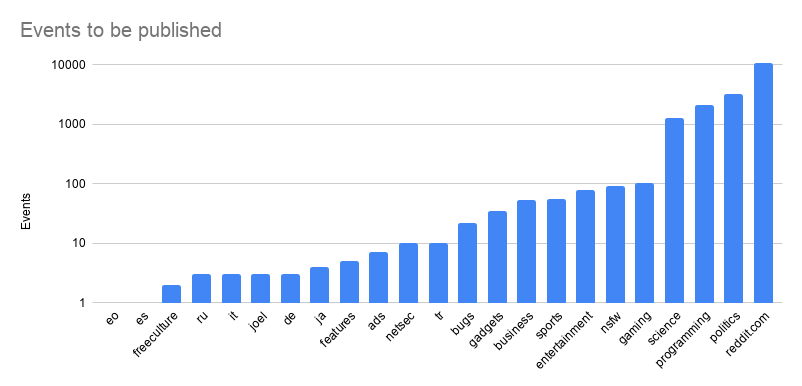
\includegraphics[width=0.8\textwidth]{img/events-to-be-publisher-per-topic.png}
  \caption{Event distribution per topic with log scale}
  \label{fig:events-to-be-publisher-per-topic}
\end{figure}

\begin{figure}[!htb]
  \centering
  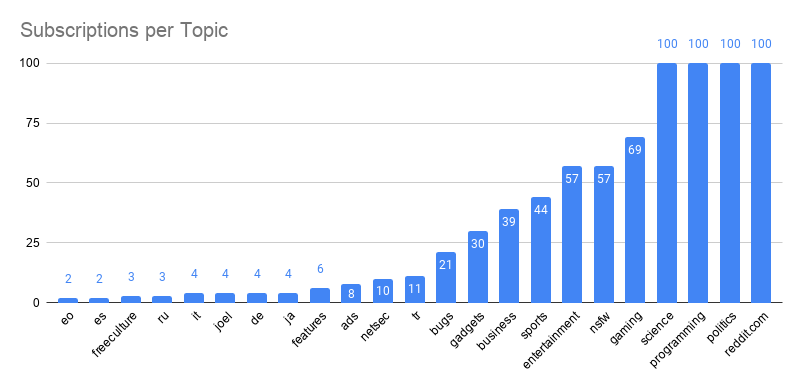
\includegraphics[width=0.8\textwidth]{img/subscriptions-per-topic.png}
  \caption{Subscription distribution per topic}
  \label{fig:subscriptions-per-topic}
\end{figure}

\begin{figure}[!htb]
  \centering
  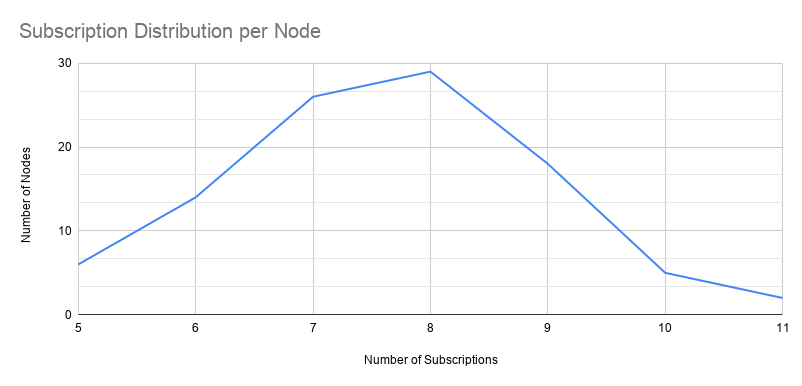
\includegraphics[width=0.8\textwidth]{img/subscription-distribution-per-node.png}
  \caption{Subscription distribution per number of nodes}
  \label{fig:subscription-distribution-per-node}
\end{figure}

\section{Metrics}\label{metrics}

For each execution we look to extract two key groups of data. Resource usage
data and QoS data. The following list describes these in more detail:

\begin{itemize}
  \item Resource usage as a total in the whole cluster, and per node (95/99
  percentile and average)
  \begin{itemize}
    \item CPU Usage (CPU number)
    \item Memory Usage (GiB)
    \item Network Usage (MiB transmitted)
  \end{itemize}
  \item QoS
  \begin{itemize}
    \item Events published by topic and in total
    \item Events received by topic and in total
    \item Percentage of subscriptions fulfilled based on the number of events
    successfully published
    \item Percentage of subscriptions fulfilled based on the number of events
    initially injected in the system
    \item Number of RPC messages sent per topic and in total
    \item Average, standard deviation and percentiles (99/95) of RPC messages
    sent by node
  \end{itemize}
\end{itemize}

It's important to keep in mind that some of the metrics under the QoS group
only make sense in Pulsarcast test runs, hence will be ignored when running the
baseline Floodsub solution.

\section{Executions}\label{executions}

We have devised a total of 6 test executions we wanted to go through and
compare results. Starting with the 3 base scenarios we wanted to test:

\begin{itemize}
  \item Pulsarcast without order delivery guarantee
  \item Pulsarcast with order delivery guarantee
  \item Floodsub (baseline solution)
\end{itemize}

For the first one, we run a scenario where every created topic in
Pulsarcast allows every participating node to publish events. For the second
execution, we configure the topics so that only the creator of the topic is
allowed to publish, all the events from other nodes will need to be forwarded
as a request to publish (as described in
\ref{subsec:publishing-and-event-dissemination}). Floodsub was used as it is,
as no configuration is required. 

For each of the executions described above, we performed two tests, one without
any network disturbances, and another using Toxiproxy's features, adding a
latency of 500 milliseconds and 300 milliseconds of jitter to every incoming
TCP packet. 

\section{Results}\label{results}

In this section we will evaluate the results for each of the executions we
described, followed by a comparison of these.

\subsection{Pulsarcast With Order Guarantee}\label{subsec:pulsarcast-with-order-guarantee}

For this test we explored how the Pulsarcast system performed when only a
single node (the creator of the topic), was allowed to effectively publish
events. The execution took a total of 38 minutes, however, at the 10 minute
mark, one of our nodes (the root node for the reddit.com topic) became
unresponsive due to the load it was dealing with and the lack of CPU power to
handle it, eventually leading the Kubernetes scheduler to restart it.  Given
that Pulsarcast does not provide a recovery mechanism for root nodes for a
topic out of the box and the fact that this was the only node allowed to
publish, we ended up seeing a clear impact in our results.

\begin{figure}[!htb]
  \centering
  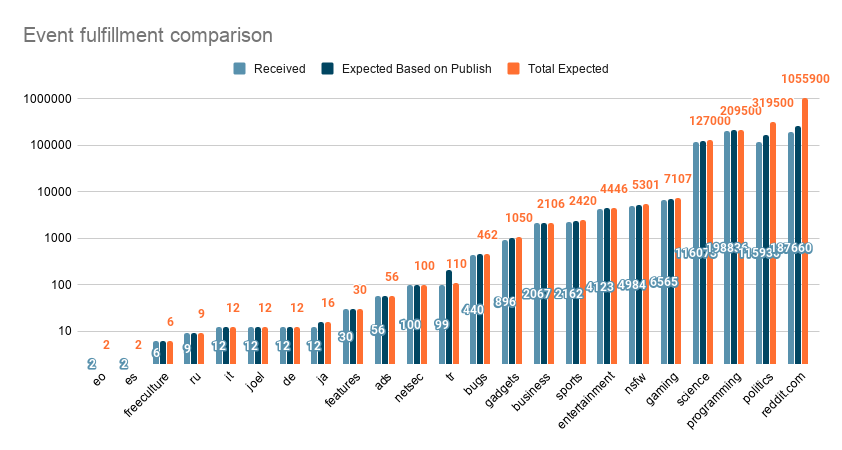
\includegraphics[width=0.8\textwidth]{img/graph-pulsarcast-order-event-fulfillment-comparison.png}
  \caption{Comparison of of events fulfilled by topic in a log scale}
  \label{fig:graph-pulsarcast-order-event-fulfillment-comparison}
\end{figure}

\begin{figure}[!htb]
  \centering
  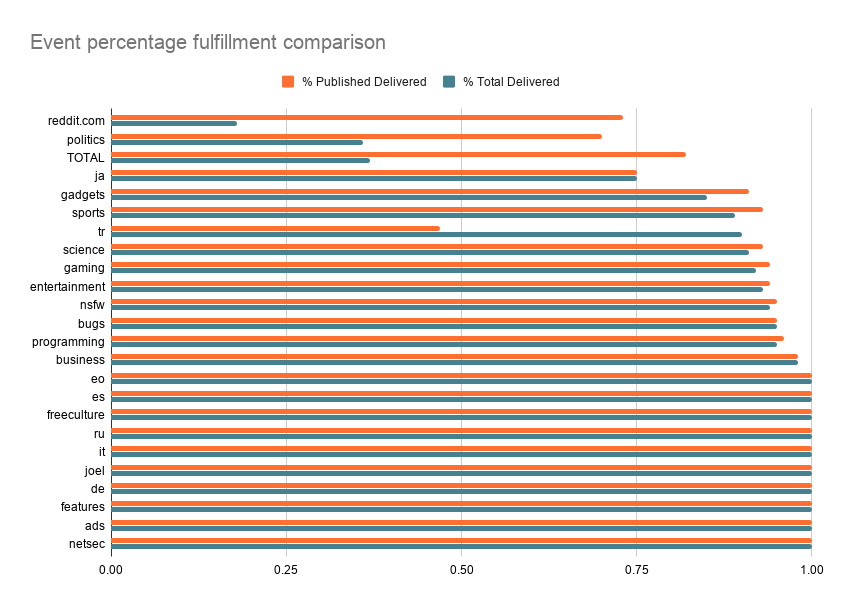
\includegraphics[width=0.8\textwidth]{img/graph-pulsarcast-order-event-percentage-fulfillment-comparison.png}
  \caption{Comparison of percentage of events fulfilled by topic}
  \label{fig:graph-pulsarcast-order-event-percentage-fulfillment-comparison}
\end{figure}

Looking at \ref{fig:graph-pulsarcast-order-event-fulfillment-comparison} and
\ref{fig:graph-pulsarcast-order-event-percentage-fulfillment-comparison} we can
see that, of the total of events injected into the system, Pulsarcast fulfilled 37\% of
its subscriptions. For the events events published, Pulsarcast fulfilled 80\%
of its subscriptions. The biggest contributors for these lower percentages were
the reddit.com and the politics topic, effectively due to the drop-out node.

\begin{figure}[!htb]
  \centering
  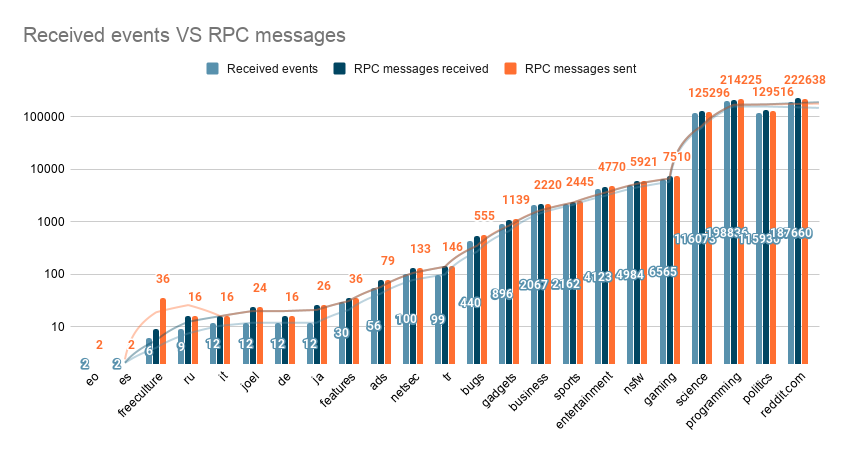
\includegraphics[width=0.8\textwidth]{img/graph-pulsarcast-order-rpc.png}
  \caption{Comparison of events received and RPC injected in the system}
  \label{fig:graph-pulsarcast-order-rpc}
\end{figure}

Considering figure \ref{fig:graph-pulsarcast-order-rpc}, we see that the RPC
messages injected in the system grow linearly with the number of events
received.

Table \ref{table:pulsarcast-order} provides an overview of the Memory and
Network utilisation by node. Given these grew linearly throw the test execution
we are only presenting the final values. We also provide an RPC message
analysis by node. Despite having a low consumption overall (Network and Memory
wise), we can see the presence of a relatively large set of outliers, a
possible consequence of the unfairness of this execution, given its tendency to
overload the owners of the topics. Now, looking at graph
\ref{fig:graph-pulsarcast-order-cpu} which shows us the CPU usage across time,
we can see the same outlier pattern as before, as well as the moment (at the 10
minute mark) when the CPU usage picked for the node which eventually became
unresponsive.

\begin{table}[!htb]
\caption{Resource utilisation metrics}
\label{table:pulsarcast-order}
  \begin{center}
   \begin{tabular}{|c| c c c c|} 
    % \label{tab:pulsarcast-order}
   \hline
   / & P95 & P99 & Average & Total \\ [0.5ex] 
   \hline\hline
   Memory (GiB) & 0.207 & 0.358 & 0.178 & 17.84 \\
   \hline
   Network (MiB) & 26.26 & 99.41 & 10.5 & 1050.4 \\
   \hline
   RPC Messages Received & 8440 & 8961 & 7315.18 & [NA] \\
   \hline
   RPC Messages Sent & 33655.5 & 80058.5 & 5889.29 & [NA] \\ [1ex] 
   \hline
  \end{tabular}
  \end{center}
\end{table}

\begin{figure}[!htb]
  \centering
  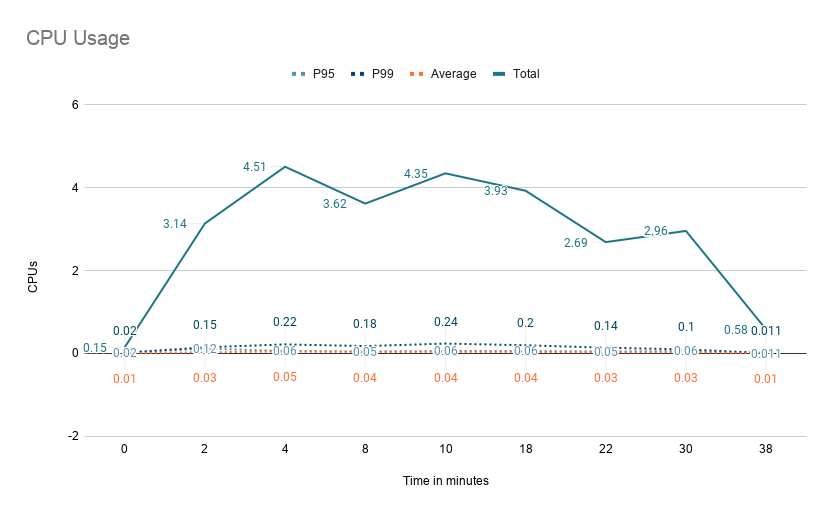
\includegraphics[width=0.8\textwidth]{img/graph-pulsarcast-order-cpu.png}
  \caption{CPU usage across time}
  \label{fig:graph-pulsarcast-order-cpu}
\end{figure}

\subsection{Pulsarcast Without Order Guarantee}\label{subsec:pulsarcast-without-order-guarantee}

We will now be looking at the Pulsarcast scenario without order guarantee,
which means, every node is able to publish messages to topics it is subscribed
to. For this scenario, the execution took a total of 85 minutes.

\begin{figure}[!htb]
  \centering
  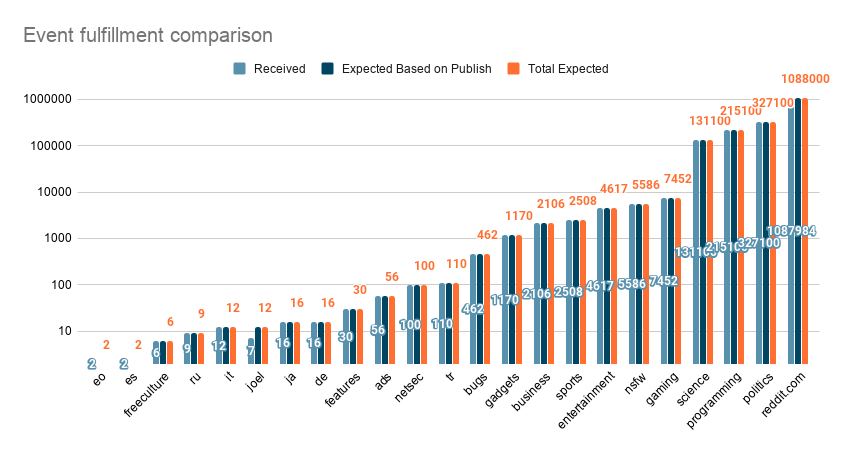
\includegraphics[width=0.8\textwidth]{img/graph-pulsarcast-event-fulfillment-comparison.png}
  \caption{Comparison of of events fulfilled by topic in a log scale}
  \label{fig:graph-pulsarcast-event-fulfillment-comparison}
\end{figure}

\begin{figure}[!htb]
  \centering
  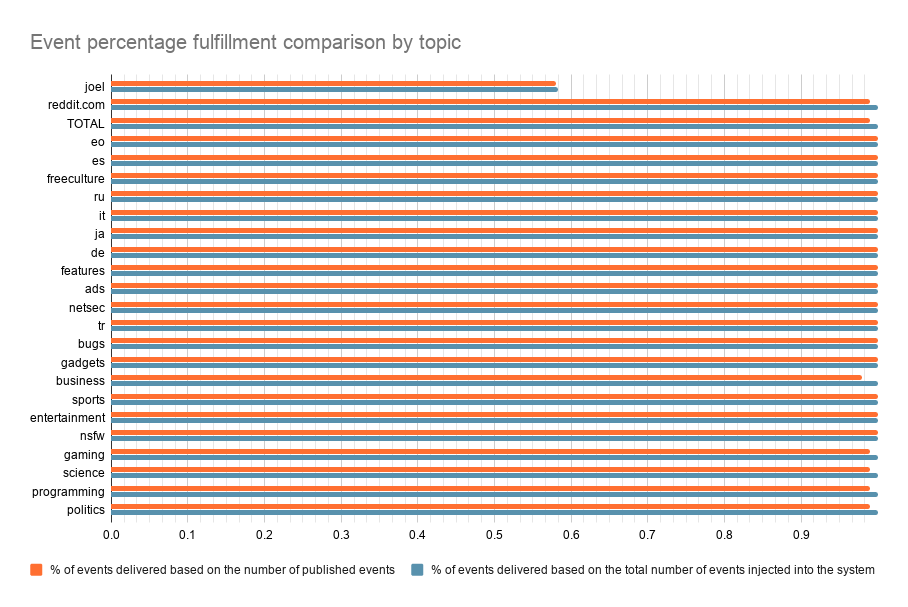
\includegraphics[width=0.8\textwidth]{img/graph-pulsarcast-event-percentage-fulfillment-comparison.png}
  \caption{Comparison of percentage of events fulfilled by topic}
  \label{fig:graph-pulsarcast-event-percentage-fulfillment-comparison}
\end{figure}

Looking at \ref{fig:graph-pulsarcast-event-fulfillment-comparison} and
\ref{fig:graph-pulsarcast-event-percentage-fulfillment-comparison} we can
see that, of the total of events injected into the system, Pulsarcast fulfilled
99\% of
its subscriptions. As for the events events published, Pulsarcast fulfilled 99\%
of its subscriptions. A clear difference to the order guarantee execution.

\begin{figure}[!htb]
  \centering
  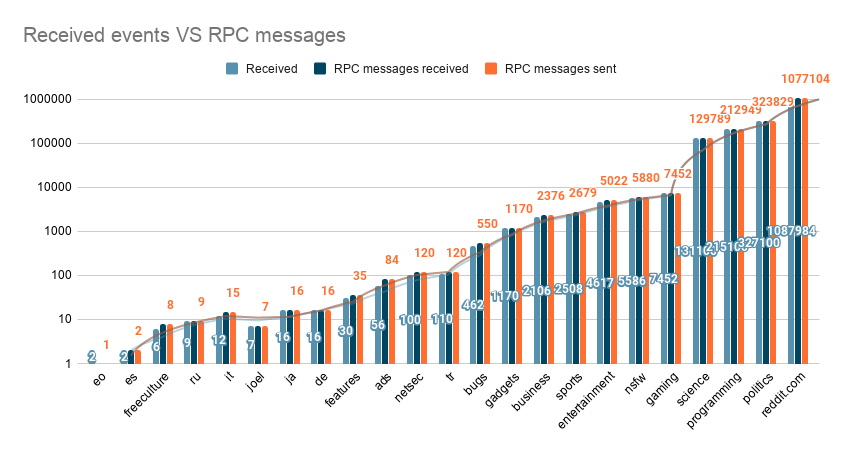
\includegraphics[width=0.8\textwidth]{img/graph-pulsarcast-rpc.png}
  \caption{Comparison of events received and RPC injected in the system}
  \label{fig:graph-pulsarcast-rpc}
\end{figure}

Considering figure \ref{fig:graph-pulsarcast-rpc}, we see that the RPC
messages injected in the system grow linearly with the number of events
received.

Table \ref{table:pulsarcast} provides an overview of the Memory and Network
utilisation by node. As previously, these grew linearly throw the test
execution we are only presenting the final values. We also provide an RPC
message analysis by node. Memory wise, we have an evenly distributed
consumption across nodes. In terms of network we still have a couple of
outliers, which can probably be explained by how the dissemination trees were
formed.  Now, looking at the graph \ref{fig:graph-pulsarcast-cpu} which shows
us the CPU usage across time, we can see a low CPU usage in total, with a small
set of outliers across time as these were the nodes publishing events at the
time (explainable due to our heavy dependency on cryptographic hash functions).
Overall though we see a clear difference in how resource consumption is more
evenly distributed compared to the order guarantee experiment.

\begin{table}[!htb]
\caption{Resource utilisation metrics}
\label{table:pulsarcast}
  \begin{center}
   \begin{tabular}{|c| c c c c|} 
    % \label{tab:pulsarcast-order}
   \hline
   / & P95 & P99 & Average & Total \\ [0.5ex] 
   \hline\hline
   Memory (GiB) & 0.369 & 0.378 & 0.319 & 31.924 \\
   \hline
   Network (MiB) & 49.143 & 129.82 & 22.377 & 2237.736 \\
   \hline
   RPC Messages Received & 17843 & 17889.5 & 17708.4 & [NA] \\
   \hline
   RPC Messages Sent & 84055 & 267124.5 & 17708.4 & [NA] \\ [1ex] 
   \hline
  \end{tabular}
  \end{center}
\end{table}

\begin{figure}[!htb]
  \centering
  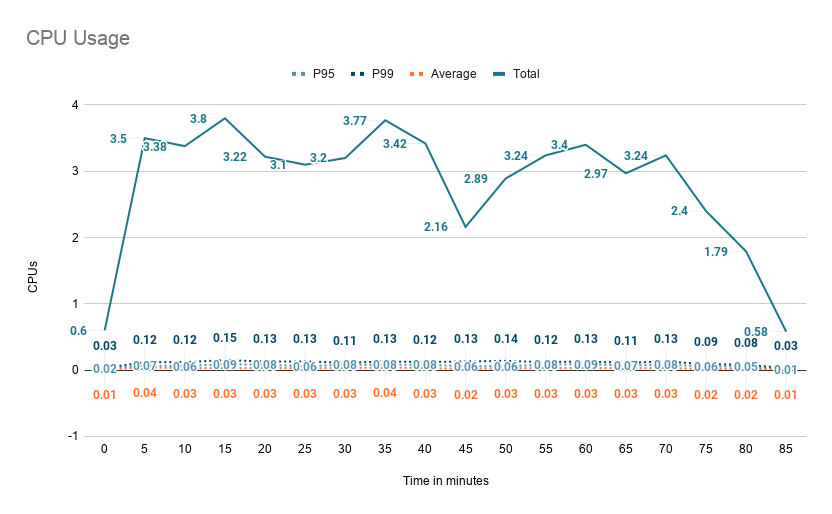
\includegraphics[width=0.8\textwidth]{img/graph-pulsarcast-cpu.png}
  \caption{CPU usage across time}
  \label{fig:graph-pulsarcast-cpu}
\end{figure}

\subsection{Floodsub}\label{subsec:floodsub}

Our next execution is a test run using Floodsub. The main goal of it is to act
as baseline for our system. Taking a total of 70 minutes to finish, the whole
network was unable to cope with the load of our execution and 10 minutes after
our test started nodes became unresponsive and either crashed or were
repeatedly terminated by our Kubernetes scheduler, eventually hitting a minimum
of 15 nodes running. It took 50 minutes for the network to fully recover and
have 100 nodes running again, only for the execution to finish 10 minutes
later.

\begin{figure}[!htb]
  \centering
  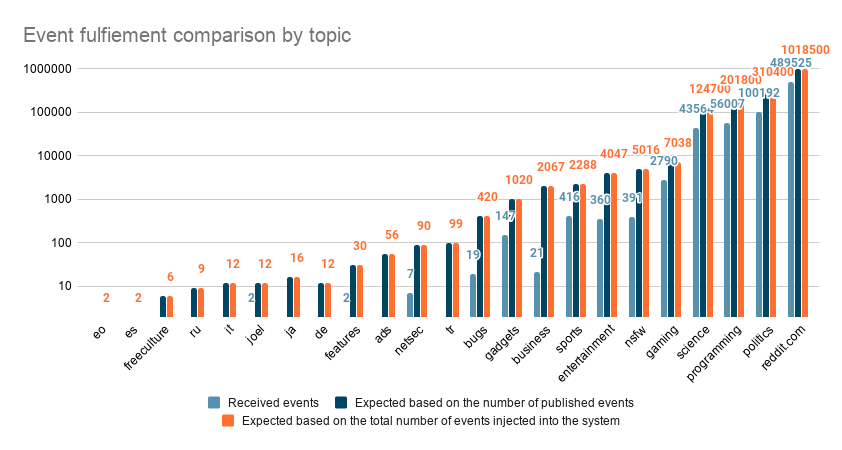
\includegraphics[width=0.8\textwidth]{img/graph-floodsub-event-fulfillment-comparison.png}
  \caption{Comparison of of events fulfilled by topic in a log scale}
  \label{fig:graph-floodsub-event-fulfillment-comparison}
\end{figure}

\begin{figure}[!htb]
  \centering
  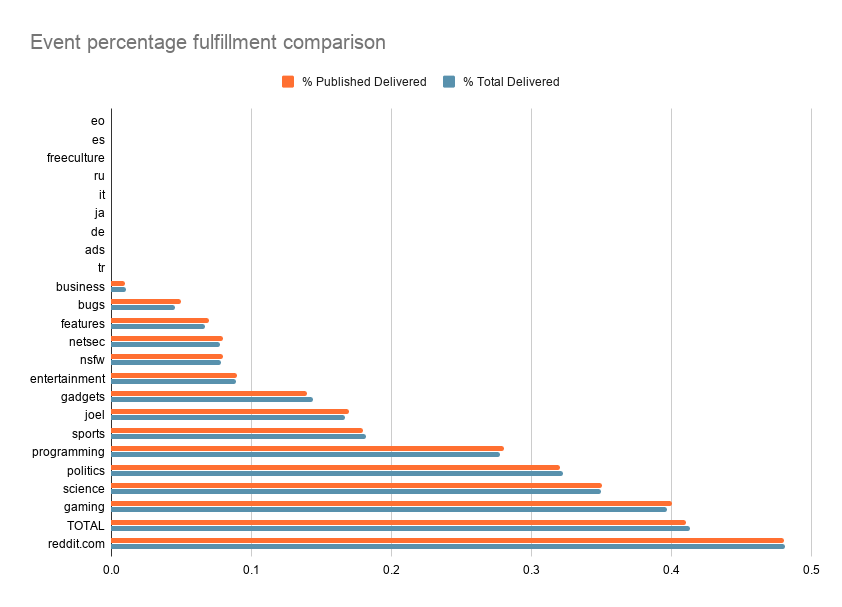
\includegraphics[width=0.8\textwidth]{img/graph-floodsub-event-percentage-fulfillment-comparison.png}
  \caption{Comparison of percentage of events fulfilled by topic}
  \label{fig:graph-floodsub-event-percentage-fulfillment-comparison}
\end{figure}

Looking at \ref{fig:graph-floodsub-event-fulfillment-comparison} and
\ref{fig:graph-floodsub-event-percentage-fulfillment-comparison} we can see
that, of the total of events injected into the system, Floodsub fulfilled 41\%
of its subscriptions. The same goes if we consider the events successfully
published as the base reference. Analysing these values, we can see they are a
little bit higher than how Pulsarcast with order guarantee performed but way
lower than base Pulsarcast test. Another thing to take into account is the way
Floodsub performed on a per topic basis, failing to fulfil a  whole range of
low popularity topics, a clear consequence of the way the whole network
crashed.

Table \ref{table:floodsub} provides an overview of the Network utilisation by
node. It grew linearly throw the test execution and as such we are only
presenting the final values. Memory wise, contrary to previous executions, it
fluctuated during the test (caused by the node failures) as such we are
presenting these values in the form of a graph in
\ref{fig:graph-floodsub-memory}. The CPU usage can be seen in
\ref{fig:graph-floodsub-cpu}. Starting by analysing the network usage, we see a
a total value of 6552 MiB transmitted, averaging at 66 MiB by node. This comes
as no surprise, given Floodsub's algorithm which repeatedly retransmits the
same event to all the peers each node is connected to. Now, looking at both the
memory and CPU evolution across time, these clearly suffered from the node
crashes. However, looking at the CPU usage, we see a total resource consumption
greater than previous executions, as well as a more uniform distribution across
nodes than for example the Pulsarcast order guarantee execution. With a P99
sometimes greater than 0.2, this explains the node failures across the test.

\begin{table}[!htb]
\caption{Resource utilisation metrics}
\label{table:floodsub}
  \begin{center}
   \begin{tabular}{|c| c c c c|} 
    % \label{tab:pulsarcast-order}
   \hline
   / & P95 & P99 & Average & Total \\ [0.5ex] 
   \hline\hline
   Network (MiB) & 105.29 & 133.9 & 65.52 & 6552.4 \\
   \hline
  \end{tabular}
  \end{center}
\end{table}

\begin{figure}[!htb]
  \centering
  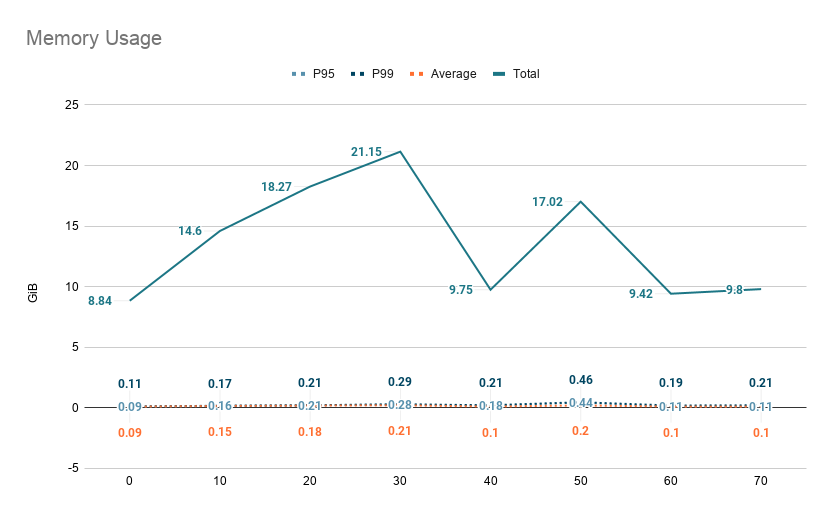
\includegraphics[width=0.8\textwidth]{img/graph-floodsub-memory.png}
  \caption{Memory usage across time}
  \label{fig:graph-floodsub-memory}
\end{figure}

\begin{figure}[!htb]
  \centering
  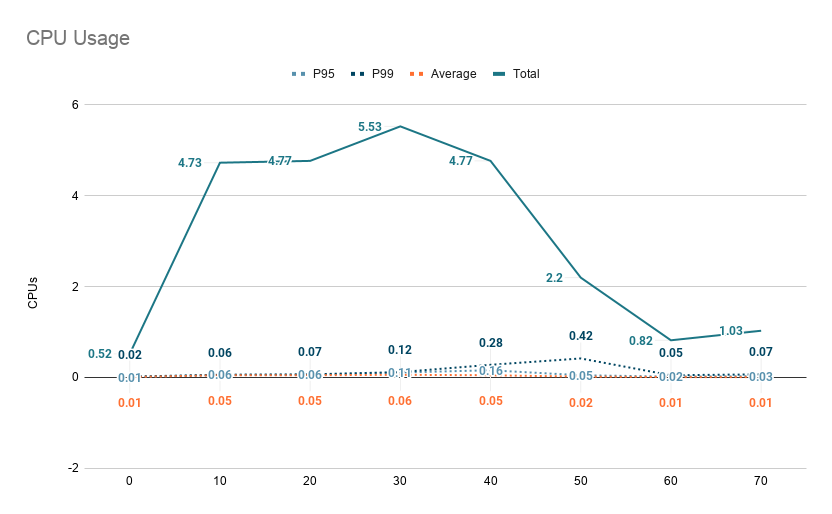
\includegraphics[width=0.8\textwidth]{img/graph-floodsub-cpu.png}
  \caption{CPU usage across time}
  \label{fig:graph-floodsub-cpu}
\end{figure}

\subsection{Pulsarcast With Order Guarantee and Latency}\label{subsec:pulsarcast-with-order-guarantee-and-latency}

\subsection{Pulsarcast Without Order Guarantee and Latency}\label{subsec:pulsarcast-without-order-guarantee-and-latency}

\subsection{Floodsub With Latency}\label{subsec:floodsub-with-latency}

\subsection{Comparison and Discussion}\label{subsec:comparison}
